\chapter{Backend}

The backend of \textbf{Think-In} is logically split into two pieces and so this chapter will be split into two subsections where each piece will be talked about in more detail. One of the logical entities of the backend is the EC2 virtual machine running a HTTP server where communication is done through the WebSocket protocol. The other logical entity is where the HTTP triggered Lambda functions reside, this entity serves as the API of the application. 

\section{The server that handles in real-time communication}

This server handles stage movements and chat messages in an event-driven and very quick way thanks to the WebSocket\footnote{\href{https://developer.mozilla.org/en-US/docs/Web/API/WebSockets\_API}{https://developer.mozilla.org/en-US/docs/Web/API/WebSockets\_API}}  communication protocol and the Socket.IO\footnote{\href{https://socket.io/}{https://socket.io/}} library. Justification for choosing the Socket.IO library is that it can fallback to HTTP polling in case communication through websockets can't be done, as well as providing abstractions that help in accelerating the development process such as: liveness detection 
and maintenance, reconnection in case of errors, encoding sent data as JSON and rooms.

\subsection{Project structure}

Just like in the previous chapter where I have talked about the frontend I will talk about the organization of files and directories and detail certain files. The file hierarchy is shown in Figure \ref{figure:backend-stage-server-project-structure}. We have met the \textit{buildspec.yml}, \textit{tsconfig.json}, \textit{.eslintrc.json} and \textit{.prettierrc.yaml} files in the frontend, they serve the same purpose here so talking about them again is unnecessary. The \textit{appspec.yml} file contains configurations for CodeDeploy and the \textit{scripts} directory contains the scripts ran by CodeDeploy, these have been detailed in the infrastructure chapter. Exploring the files in \textit{src/}, the \textit{socketio} directory contains files whose logic handles chat and stage interactions, more precisely code in \textit{chats.ts} manages chat messages and the code in \textit{stages.ts} handles stage interactions. Eagle-eyed readers will find a correlation between these two files and the \textit{ChatManager} and \textit{AttenderManager} components in the frontend, that's no coincidence because code in these two files emit the events handled by the two components. \textit{socketIOServer.ts} aggregates the code in these two files and creates a HTTP server to be used in the \textit{src/index.ts} file. The \textit{types/} directory contains type declarations that simply augment the dependency type declarations. In the \textit{utils/sesEmail} directory we find one HTML email template and one plain text email template as well as code using the AWS SES\footnote{\href{https://aws.amazon.com/ses/}{https://aws.amazon.com/ses/}} service. The \textit{src/index.ts} serves as the entry point of the application and the \textit{src/shared.ts} file contains common code utilized throughout the application.

\begin{figure}[H]
\begin{verbatim}
STAGE_SERVER
|- buildspec.yml
|- appspec.yml
|- tsconfig.json
|- .eslintrc.json
|- .prettierrc.yaml
|- node_modules/
|- scripts/
|- src/
   |- socketio/
      |- chats.ts
      |- stages.ts
      |- socketIOServer.ts
   |- types/
   |- utils/
   	  |- sesEmail/
   	     |- email.txt
   	     |- email.html
   	     |- sesEmail.ts   
   |- index.ts
   |- shared.ts  
\end{verbatim}
\caption{Backend server project structure.}
\label{figure:backend-stage-server-project-structure}
\end{figure}

\subsection{Decoupled logic}

Going forward I would like to detail the \textit{src/socketIOServer.ts} file. I have purposely stripped code in order to improve readability. Here an implementation of the Chain of Responsibility\footnote{\href{https://en.wikipedia.org/wiki/Chain-of-responsibility\_pattern}{https://en.wikipedia.org/wiki/Chain-of-responsibility\_pattern}} pattern was used, which is made visible between lines 4-20 in Figure \ref{figure:backend-stage-server-socketIOServer-file} where the authorization of a user is done based on whether or not the provided JWT upon socket connection is valid or not. In the \textit{createSocketIOServer} function we simply attach the middleware and listeners to the server instace (represented by the \textit{io} variable here}. Observe how the stage and chat listeners are in no way dependent upon each other, this can be useful when only one of these functionalities is wanted. Even more, these functionalities can be split among servers, therefore achieving easier scalability on an exact feature.

\begin{figure}[H]
\begin{lstlisting}[numbers=left,language=JavaScript]
import registerStageListeners from './stages';
import registerChatListeners from './chats';

const registerGeneralMiddleware = (io: SocketIOServer) => {
  ['/stages', '/chats'].forEach((namespace) => {
    io.of(namespace).use(async (socket, next) => {
      try {
        const idTokenDecoded = 
          await validateJWT(socket.handshake.auth.idToken as string);
        socket.idToken = socket.handshake.auth.idToken;
        socket.idTokenDecoded = idTokenDecoded;
        socket.attender =
          JSON.parse(socket.handshake.query.attender as string);
        next();
      } catch (e) {
        next(new Error('Not authenticated.'));
      }
    });
  });
};

const createSocketIOServer: CreateSocketIOServer = (httpServer) => {
  const io = new SocketIOServer(httpServer, socketIOOptions);

  registerGeneralMiddleware(io);
  registerStageListeners(io);
  registerChatListeners(io);

  return io;
};
\end{lstlisting}
\caption{Backend \textit{socketIOServer.ts} file}
\label{figure:backend-stage-server-socketIOServer-file}
\end{figure}

\subsection{Handling messages}

Sending the message when both the originator and the receiver of the message are online is trivial, the server simply relays the message to the receiver. However, this logic gets more complex when the receiver is offline. The code that is executed whenever a message is sent is shown in Figure \ref{figure:backend-stage-server-messages}, changes regarding comments, formatting and removing requests headers were made to it in order to fit in the page. Lines 2-6 deals with messages sent to the Global/Stage chat, these two chats are perceived as special users and are always considered online. Lines 6-24 manage messages sent to users in the following way: the condition at line 8 is equivalent to checking if the user is online, if so simply relay the message, however if the user is offline we wish to inform him of the message via email, as well as notify him next time he opens the application. In case he receives more messages from a single user, we want to avoid sending multiple emails to the user and instead send a single email informing the user of multiple potential messages. This logic is implemented between lines 12-25. Finally, lines 29-31 persist the message to the database so they can be retrieved even through client sessions.

\begin{figure}[H]
\begin{lstlisting}[numbers=left,basicstyle=\small,language=JavaScript]
// toUser, message, isGlobalOrStageChat are sent by the client
if (isGlobalOrStageChat) {
  // message was meant for the global or stage chat
  io.of('/chats').in(toUser.id).except(socket.id)
    .emit('private-message', { message, fromUser: toUser });
} else {
  // message was meant for a user, check if the user is online
  if (userIdToSocketIdMap.has(toUser.id)) {
    // toUser is online, directly send message
    socket.to(userIdToSocketIdMap.get(toUser.id) as string)
          .emit('private-message', { message, fromUser: socket.attender });
  } else {
    // toUser is offline
    
    // send email to user regarding this message only if this is the first
    // unread message
    // verify there are no other unread messages before sending email
    const response = await axios.get(`${API_URL}/notifications/${toUser.id}`);
    if (response.data.data.items.length === 0)
        await sendEmail({ destinationEmail: toUser.email,
          fromUser: socket.attender, message });

    // save notification to DB
    await axios.post(`${API_URL}/notifications/${toUser.id}`, socket.attender);
  }
}

// save message to DB
const url = new URL(`${API_URL}/chats/
    ${computeChatId(toUser.id, socket.attender.id)}`);
await axios.post(url.toString(), message);
\end{lstlisting}
\caption{Handling messages.}
\label{figure:backend-stage-server-messages}
\end{figure}

The above logic applies whether the message is plain text or media. Now let's see how sending plain text messages differs from sending media messages. Sending a plain text message is straightforward both for the user and also from the developer's point of view, an event is emitted from the client with the data of the plain text message. Sending a media message however implies more than one single round trip, a sequence diagram\footnote{\href{https://en.wikipedia.org/wiki/Sequence\_diagram}{https://en.wikipedia.org/wiki/Sequence\_diagram}} is shown in Figure \ref{figure:backend-stage-server-media-message} which shows the interactions needed in order to send one such message.

\begin{figure}[H]
	\centering
	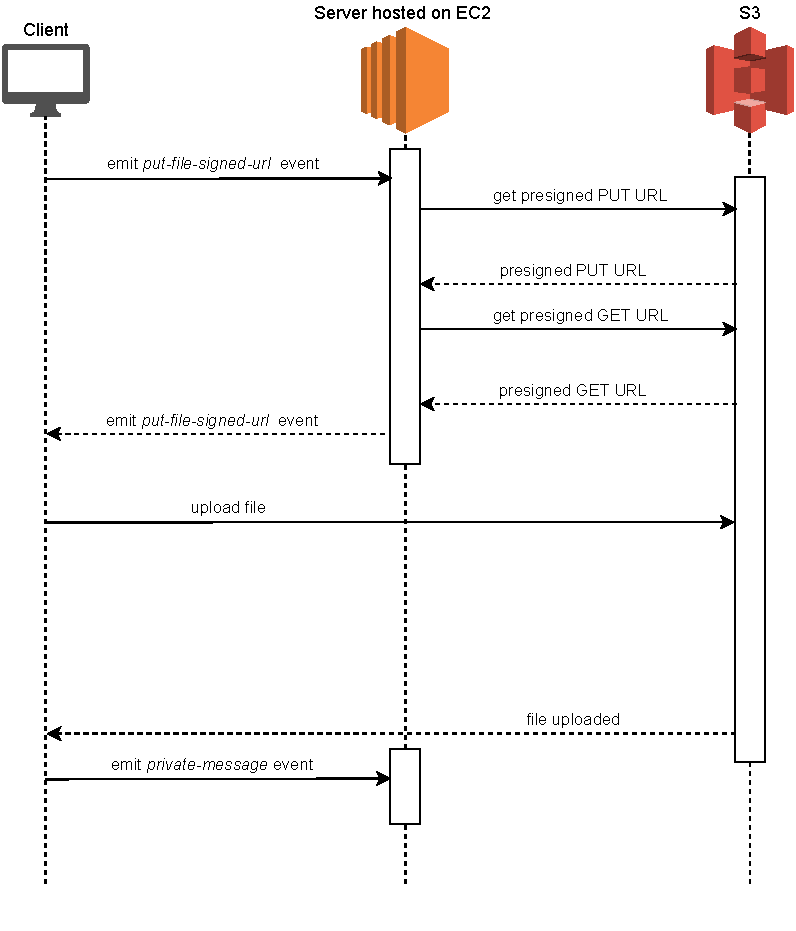
\includegraphics[width=\textwidth,keepaspectratio]{images/backend/upload-media.pdf}
	\caption{Interactions necessary for uploading media.}
	\label{figure:backend-stage-server-media-message}
\end{figure}

As seen from the diagram, the client uploads the file directly to S3. In order to do so, the client first asks the backend server for a presigned PUT URL, used for uploading the photo, and a presigned GET URL, which is valid only for a day and used later in order to send the message in the chat. Had I learned about Cognito Identity before doing this it could have been done differently, the client could get authorization credentials straight from Cognito and the entire communication with the server before uploading the file would be omitted.

\subsection{Securing messages}

For securing plain text messages, access to the API is granted only to those who are participants of a chat. First of all the JWT is verified and if valid then it is checked whether or not the participants of the chat include that user, if so then the user is authorized.

The media messages are stored in a private S3 bucket and they are not accessible to the public. For retrieving messages from a chat the server is asked to do so, the server then gets them from the API and presigns media messages' URLs after which the links to media are valid for one day (can be changed to any amount of time). Advantages are that, if the user wishes so, he can share the link to the media to non-participants of the chat. A disadvantage to this approach is that the server is involved, by the time I realized this could be done with a request to a HTTP triggered function the logic was already implemented.

\subsection{Using HTTPS}

Because there can be private data transported the server had to be secured.
The way I achieved the server to run over HTTPS is somewhat unexpected. Another way I think this could have been done is by getting a certificate authority\footnote{\href{https://en.wikipedia.org/wiki/Certificate\_authority}{https://en.wikipedia.org/wiki/Certificate\_authority}} such as Let's Encrypt\footnote{\href{https://letsencrypt.org/}{https://letsencrypt.org/}} to issue a digital certificate, use it to host a HTTPS server instead and add a DNS CNAME record to point to the EC2 instance hostname. However, this was achieved by using an Application Load Balancer\footnote{\href{https://aws.amazon.com/elasticloadbalancing/application-load-balancer/}{https://aws.amazon.com/elasticloadbalancing/application-load-balancer/}} as AWS provides communication over HTTPS to the load balancer. The load balancer essentially acts as a proxy server, as seen in Figure \ref{figure:backend-stage-server-https}. An advantage of doing this was that a load balancer needed to be set up for greater scalability anyway.

\begin{figure}[H]
	\centering
	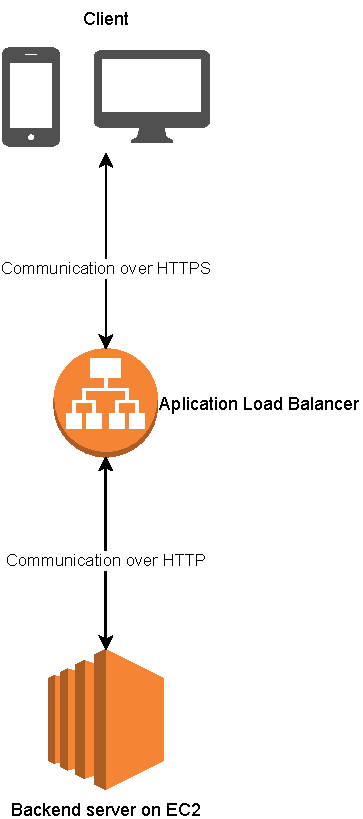
\includegraphics[width=.5\textwidth,keepaspectratio]{images/backend/server-proxy.pdf}
	\caption{How the ALB\footnote{Application Load Balancer} acts a TLS termination proxy\footnote{\href{https://en.wikipedia.org/wiki/TLS\_termination\_proxy}{https://en.wikipedia.org/wiki/TLS\_termination\_proxy}}}
	\label{figure:backend-stage-server-https}
\end{figure}


\section{REST API}

As seen and talked about in the architecture chapter the REST API is created from HTTP triggered AWS Lambda functions whose access are centralized by an AWS API Gateway, which essentially acts as a reverse proxy. For persisting the data I chose AWS DynamoDB\footnote{\href{https://aws.amazon.com/dynamodb/}{https://aws.amazon.com/dynamodb/}} as that is a managed solution as well.

\subsection{Project structure}

The file and directories hierarchy here is the easiest to understand compared to the other ones. The first four files/directories have been explained before. The \textit{serverless.yaml}  file is Serverless\footnote{\href{https://serverless.com/}{https://serverless.com/}} specific and contains IaC\footnote{Infrastructure as Code} that deploys all the necessary resources with their configurations, as talked about in the infrastructure chapter. The \textit{OPENAPI.yaml} file contains an API specification that makes it easier to describes and visualize the services providen by the \textbf{Think-In} API, it is written according to the OpenAPI Specification\footnote{\href{https://swagger.io/specification/}{https://swagger.io/specification/}}. The \textit{shared.ts} file contains code that is common across this application. In the last six directories every file corresponds to a HTTP triggered Lambda function. In the \textit{avatars} directory the \textit{post-avatar-token.ts} file contains logic that resizes and changes the user avatar when the user passes a token, i.e. when the user is logged in and changes his avatar from the profile page. The \textit{post-avatar-id.ts} file contains logic for handling the use case when the user picks an avatar when registering, at this point the user can't be logged in and therefore can't use a token to request to the function previously explained. The hacky solution I went through is that a user can change his avatar as long as he is unconfirmed and knows his ID. The \textit{translations} directory contains logic that deals with, of course, translation. For this I have relied the burden of translating between languages to Google Translate\footnote{\href{https://en.wikipedia.org/wiki/Google\_Translate}{https://en.wikipedia.org/wiki/Google\_Translate}} because it has always been my go-to language translation app. The function in the \textit{get-languages.ts} file simply returns the languages supported by Google Translate, the function in \textit{post-translate.ts} deals with actual language translation. The last four directories contain code for functions that respect the REST architectural style constraints.

\begin{figure}[H]
\begin{verbatim}
REST_API
|- tsconfig.json
|- .eslintrc.json
|- .prettierrc.yaml
|- node_modules/
|- serverless.yaml
|- OPENAPI.yaml
|- shared.ts
|- avatars/
   |- post-avatar-id.ts
   |- post-avatar-token.ts
|- translations/
   |- get-languages.ts
   |- post-translate.ts
|- chats/
|- notifications/
|- stages/
|- users/
\end{verbatim}
\caption{Backend server project structure.}
\label{figure:backend-stage-server-project-structure}
\end{figure}

\subsection{DynamoDB design}

Before further explaining we need to have a slight idea of how DynamoDB works. It is a NoSQL database that stores items in a table, each item containing attributes, this results in schemaless items very alike JSON\footnote{\href{https://www.json.org/json-en.html}{https://www.json.org/json-en.html}} objects. DynamoDB supports two types of primary keys:
\begin{itemize}
	\item \textbf{Partition key} - items are uniquely identified by a single attribute, based on the attribute the item will be assigned to a physical partition
	\item \textbf{Partition key and sort key} (composite key) - items are uniquely identified by a combination of two attributes, the items are assigned to a physical partition by the primary key, and are sorted in that partition by the sort key.
\end{itemize}

Having this knowledge I had to study the data access patterns of the application. One particular use case that stands out is fast message retrieval, most certainly if people used \textbf{Think-In} they exchanged only a couple messages and most importantly other contact data so further talking will be done through another medium. For this reason I don't want people to wait a long amount of time to retrieve that meaningful information. In order to achieve this I didn't want time to be lost on sorting the messages between users, so the fact that DynamoDB holds the data in memory naturally sorted helped, therefore I chose to have a \textbf{partition key} and a \textbf{sort key} where a message will have the following format:
\begin{itemize}
	\item Partition key of the format \verb|chat_{chatId}|
	\item Sort key of the format \verb|message_{timestamp}_{id}|.
\end{itemize}

In doing so, if we search by the partition key we get to the physical partition where the messages are stored sorted by timestamp, that sounds fast! The justification for an  additional ID at the end of the sort key is to account for the rare case where multiple messages have the same timestamp. Knowing that DynamoDB and the Lambda function are hosted in the Frankfurt region, I got an average response time of 281 milliseconds over 15 requests. The function was initialised (i.e. it had no cold start\footnote{\href{https://www.serverless.com/blog/keep-your-lambdas-warm}{https://www.serverless.com/blog/keep-your-lambdas-warm}}) before performing the requests. In case there was any doubt, the data identified by the partition key and sort key respects the contract of the message described in the frontend chapter.


Another data that needed to persist was notifications, that is who messaged a user while he was offline, next time he logs in he should be notified of the users who left him messages. In this case a notification has the partition key of format \verb|user_{userId}| and sort key \verb|notification_{id}|. An access pattern here would be to simply get all items that have the partition key equal to that of a user's ID in order to get all his notifications, whether or not the notifications are sorted doesn't matter. The contents stored for a notification is the message sender's information so next time the receiver logs in a new chat with the sender user will be loaded.

What is stored in the database is also information about stages, the information that can be seen in the horizontally scrolling area of the index page. In this case the partition key is \verb|stages| and the sort key is \verb|{stageId}|. The information stored about a stage is the following:
\begin{itemize}
	\item title - the stage title
	\item subheader - the text shown below the stage title
	\item body - description about the entity behind the stage
	\item externalLink - an external link to more information about the entity behind the stage
	\item imageLink - a link to an image provided by the entity behind the stage
	\item videoLink - a link to a video provided by the entity behind the stage.
\end{itemize}


In retrospective, after using other managed database solutions provided by other cloud platforms (e.g. Cloud Firestore, Firebase Realtime Database), interacting with DynamoDB hasn't been the most pleasant experience from a developer's point of view. For instance having to specify query expressions using strings did not feel modern to me. Moreover, performing pagination was a headache, the traditional limit and offset parameters have been substituted by  the partition key and sort key, so everytime I wanted to obtain another page I had to specify the last retrieved item's partition key and sort key.


\subsection{Changing avatar functionality}

At the heart of changing a user's avatar sits the function in Figure \ref{figure:backend-rest-api-avatar}. As observed by lines 2-3, in order to save bandwidth and improve loading times the image is processed so that it is resized, furthermore it's brought to a common format, in this case \verb|image/jpeg|. Between lines 5-12 the new avatar is uploaded to S3, and lines 14-20 change the \textit{picture} attribute of the user so that it now points to the newest location.


\begin{figure}[H]
\begin{lstlisting}[numbers=left,basicstyle=\small,language=JavaScript]
const uploadAvatarToS3AndUpdateUserAttribute = async (userId, avatarBuffer) => 
{
  const processedAvatar = await sharp(avatarBuffer)
                                  .resize(256, 256).jpeg().toBuffer();

  const { Location: avatarURI } = await s3
    .upload({
      Bucket: process.env.S3_CHATS_BUCKET!,
      Key: `avatars/${userId}.jpg`,
      Body: processedAvatar,
      ContentType: 'image/jpeg',
    })
    .promise();

  await cognitoIdentityServiceProvider
    .adminUpdateUserAttributes({
      UserPoolId: process.env.COGNITO_USER_POOL_ID!,
      Username: userId,
      UserAttributes: [{ Name: 'picture', Value: avatarURI }],
    })
    .promise();

  return avatarURI;
};
\end{lstlisting}
\caption{Logic of changing an avatar.}
\label{figure:backend-rest-api-avatar}
\end{figure}










